\documentclass[12pt,a4paper]{book}
\usepackage{afterpage}
\usepackage{fontspec}         
\setmainfont{Arial}
\newfontfamily{\cyrillicfonttt}{Arial}
\newfontfamily{\cyrillicfont}{Arial}
\newfontfamily{\cyrillicfontsf}{Arial}
\usepackage{polyglossia}     
\setdefaultlanguage{russian}  
\setotherlanguage{english}
\usepackage[paper=a4paper,top=10mm, bottom=10mm,left=35mm,right=35mm,includefoot,includehead]{geometry}
\setlength{\parskip}{4mm}
\setlength{\parindent}{0mm}
\newcommand{\mysize}[1]  
{{\fontsize{14}{1}\selectfont #1 }}
\usepackage{graphicx}                 
\usepackage{graphics}
\usepackage{hyperref}
\hypersetup{
    unicode=true,           
    colorlinks=true,       	
    urlcolor=black}

\usepackage{fancyhdr} 
\pagestyle{fancy}
\setcounter{page}{3}
\renewcommand{\thesection}{Приложение \Asbuk{section}}
\setcounter{section}{0}
\renewcommand{\headrulewidth}{0.2pt}  
\renewcommand{\footrulewidth}{0.2pt}  
	\lfoot{}
	\rfoot{}
	\rhead{\thepage}
 	\chead{}
	\lhead{\rightmark}
	\cfoot{Школа Чародейства и Волшебства "Хогвартс"}
	
\renewcommand{\labelitemi}{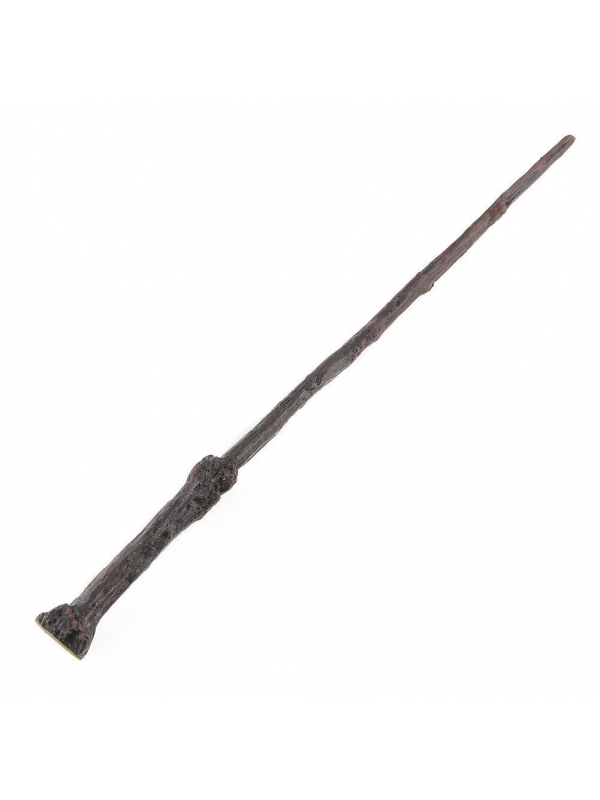
\includegraphics[scale=0.05]{palka.jpg}}


\begin{document}

\begin{titlepage}
\thispagestyle{empty}

\begin{figure}
\begin{center}

\includegraphics[height=6cm]{hogw.png}
\end{center}
\end{figure}
\vspace{1cm}

Мисс Эрдман

\vspace{2.5cm}

\mysize{Дорогая мисс Эрдман, 

Мы рады проинформировать Вас, что Вы приглашаетесь в Школу Чародейства и Волшебства "Хогвартс".

Убедительно просим Вас ознакомиться с приложенным к данному письму списком необходимых книг и предметов. 

Занятия начнутся 1 сентября. Ждём Вашу сову не позднее 31~июля.

Искренне Ваша,

{\fontspec{HeinrichScript} Minerva Mc gonogall }

Минерва МакГонагалл

заместитель директора

}

\vspace{\fill}
\begin{center}
\mysize{\href{https://www.pottermore.com/explore-the-story/hogwarts}{\textbf{Школа Чародейства и Волшебства "Хогвартс"}}}

Директор: Альбус Дамблдор\\
(Кавалер ордена Мерлина первой степени, основатель Ордена Феникса, председатель Международной Конфедерации Магов)
\end{center}

\end{titlepage}

\newpage

\section{Список необходимых книг и предметов}
\begin{itemize}
\item Волшебная палочка
\item Мантия - неидимка
\item Камень,оживляющий мёртвых
\item Блевательные батончики
\item Задачник Дамблдора
\end{itemize}
\newpage
\section{Список изучаемых предметов}
\begin{itemize}
\item Магический анализ
\item Зельеварение
\item Защита от Тёмных искусств
\end{itemize}
\end{document}
